\documentclass{report}
\usepackage{tikz}
\usetikzlibrary{automata,positioning}
\begin{document}
\begin{figure}
	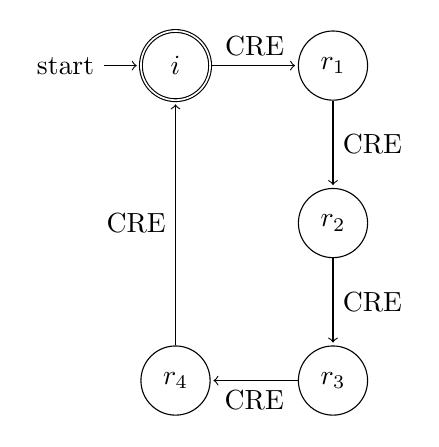
\begin{tikzpicture}[shorten >=1pt,node distance=2cm,on grid,auto]
	   \node[state,initial,accepting] (i) {$i$};
	   \node[state] [right=of i] (r_1) {$r_1$};
	   \node[state] [below=of r_1] (r_2) {$r_2$};
	   \node[state] [below=of r_2] (r_3) {$r_3$};
	   \node[state] [left=of r_3] (r_4) {$r_4$};
	   \path[->]
			(i) edge node {CRE} (r_1)
			(r_1) edge node {CRE} (r_2)
			(r_2) edge node {CRE} (r_3)
			(r_3) edge node {CRE} (r_4)
			(r_4) edge node [bend right] {CRE} (i);
	\end{tikzpicture}
\end{figure}
\end{document}
